% CHAPTER SLIDE
\cscschapter{Introduction}

%%%%%%%%%%%%%%%%%%%%%%%%%%%%%%%%%%%%
\begin{frame}[fragile]{}
%%%%%%%%%%%%%%%%%%%%%%%%%%%%%%%%%%%%
    \begin{info}{The plan}
        \begin{itemize}
            \item learn about the GPU memory model
            \item implement parallel CUDA kernels for simple linear algebra
            \item learn how to scale our parallel kernels to utilize all resources on the GPU
            \item understand which types of workloads can best take advantage of GPU resources
            \item learn about thread cooperation and synchronization in CUDA
            \item learn about concurrent task-based parallelism with CUDA
            \item learn how to use MPI in CUDA applications
        \end{itemize}
    \end{info}

\end{frame}

%%%%%%%%%%%%%%%%%%%%%%%%%%%%%%%%%%%%
\begin{frame}[fragile]{}
%%%%%%%%%%%%%%%%%%%%%%%%%%%%%%%%%%%%
    \begin{info}{Prerequisites for the course}
        \begin{itemize}
            \item no GPU or graphics experience required
            \item I assume C++ knowledge
            \begin{itemize}
                \item I will be using C++11 (the bits that make C++ easier!)
                \item there is no native CUDA implementation for Fortran
                \begin{itemize}
                    \item there is a CUDA Fortran provided by PGI, however it is not widely used.
                \end{itemize}
                \item Fortran users are encouraged to work with a C++ user for the practical exercises
            \end{itemize}
            \item the generic GPU programming concepts in the CUDA part will be useful for people interested in OpenACC
        \end{itemize}
    \end{info}

\end{frame}

%%%%%%%%%%%%%%%%%%%%%%%%%%%%%%%%%%%%
\begin{frame}[fragile]{}
%%%%%%%%%%%%%%%%%%%%%%%%%%%%%%%%%%%%
    \begin{info}{CUDA language is a superset of C++}
        \begin{itemize}
            \item write CPU code using C++ (C++11 since CUDA 6.5)
            \item keywords for writing tasks to be executed by GPU threads (kernels)
            \item use special syntax for launching tasks/kernels on GPU
        \end{itemize}
    \end{info}

    \begin{info}{CUDA is GPU-specific}
        \begin{itemize}
            \item the CUDA language extensions define the \emph{programming model}
            \item features map directly to hardware (e.g. shared memory, thread blocks)
        \end{itemize}
    \end{info}

    \begin{info}{CUDA toolkit is more than just a language}
        \begin{itemize}
            \item runtime library for managing GPU resources
            \item tools for profiling and debugging
        \end{itemize}
    \end{info}
\end{frame}


%%%%%%%%%%%%%%%%%%%%%%%%%%%%%%%%%%%%
\begin{frame}[fragile]{}
%%%%%%%%%%%%%%%%%%%%%%%%%%%%%%%%%%%%
    \begin{info}{What about the GPU in my laptop/desktop/cluster?}
        \begin{itemize}
            \item the GPUs in Piz Daint are NVIDIA Tesla K20X devices
            \item Tesla devices are high-end products with features required for high-performance computing
            \begin{itemize}
                \item high double precision performance (1.2 TFlops)
                \item large DRAM (6 GB)
                \item ECC memory
            \end{itemize}
            \item the K20X Tesla cards use the Kepler architecture
            \begin{itemize}
                \item some features are not supported by older cards
            \end{itemize}
            \item I focus on features of the K20X devices for this course
        \end{itemize}
    \end{info}

\end{frame}

%%%%%%%%%%%%%%%%%%%%%%%%%%%%%%%%%%%%
\begin{frame}[fragile]{}
%%%%%%%%%%%%%%%%%%%%%%%%%%%%%%%%%%%%
    \begin{columns}[T]
        \begin{column}{0.4\textwidth}
            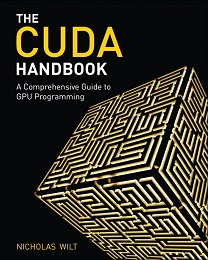
\includegraphics[width=\textwidth]{./images/CUDA-Handbook-Cover208_260.jpg}
        \end{column}

        \begin{column}{0.6\textwidth}
            \begin{info}{recommended reading}
                \textbf{\small CUDA Handbook: A Comprehensive Guide to GPU Programming}
                \begin{itemize}
                    \item  Nicholas Wilt
                    \item  released in 2013
                    \item  detailed coverage of everything you need to know
                    \item  lots of example codes and micro-benchmarks
                \end{itemize}
            \end{info}
        \end{column}
    \end{columns}
    \begin{center}
    \end{center}
\end{frame}
